The testing strategy for the S\&C platform is based on a combination of manual and automated testing techniques. Manual testing is performed by the development team to verify the correctness of the application's functionality, user interface, and user experience. Automated testing is performed using testing frameworks and tools to verify the correctness of the application's business logic, data integrity, and performance. The following sections will provide an overview of the testing strategy using during the development and the integration phase.
\subsection{Unit Testing}
For the development testing phase we mainly used JUnit and Mockito to test the backend layer of the S\&C platform. JUnit is a popular testing framework for Java that is widely used in enterprise applications, web development, and mobile applications. Mockito is a mocking framework for Java that allows developers to create mock objects for testing purposes. It is mainly used to isolate the code under test from its dependencies, such as external services, databases, and APIs.\\
Following what we already describe in the DD document, during this phase we mainly focused on testing the business logic of the application and the data integrity. This is visible in the test classes that we created for each of the main components of the S\&C platform which mainly test the CRUD operations of the different entities while postponing the test of the API end-points and the DTO classes to the integration testing phase. 

\begin{figure}[H]
    \centering
    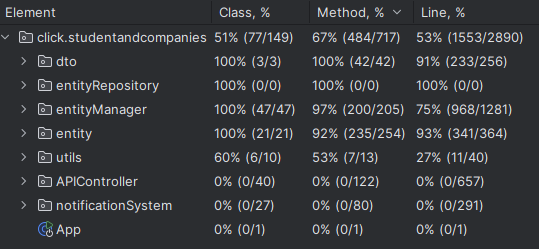
\includegraphics[width=0.5\linewidth]{Latex/Images/ITD/Coverage.png}
    \caption{Coverage result}
    \label{fig:coverage}
\end{figure}

\subsection{Integration Testing}
For the integration testing phase we mainly used Postman as a "Proxy Driver" to test the RESTful APIs created with Spring Boot following the same strategy describe in the DD document at the 3° testing step. The main goal of this phase is to verify that the different components of the S\&C platform work together correctly and that the data flow between them is consistent and reliable. The integration testing phase is performed by the development team to identify and fix any issues related to the interaction between the call made by the frontend and the computation made by the backend and the database. We created more than 30 different API call that were later used in Postman unit suite, that allowed us to test all the different functionalities of the platform, from the user registration to the internship creation, from the recommendation process to the interview management.\\
Postman allowed us to randomize request parameters and body content to test the system's robustness and evaluate different edge cases that could arise during normal platform usage. Examples include creating an internship with a missing field, accepting a recommendation that has already been approved, or attempting to fetch a non-existent internship and much more. The integration testing phase is essential to ensure that the S\&C platform works as expected, all the functionalities are implemented correctly, and the right exceptions are thrown when the user tries to perform an invalid operation.
%insert here postman call screenshot